% !Mode:: "TeX:UTF-8"
%% 请使用 XeLaTeX 编译本文.
\documentclass[forlib]{HDUMaster}   % 选项 forprint: 交付打印时, 建议加上此选项, 以消除彩色链接文字, 避免彩色字迹打印偏淡.
                                              % 选项 forlib: 提交给图书馆的电子版, 需要加上选项 forlib, 以消除空白页和彩色链接.
                                              % 选项 smd: Specialist Master's Degree, 产生专业硕士学位论文封面、页眉.
%%%=== 参考文献=== %%%
\bibliographystyle{abbrv}        % 参考文献样式,  plain,unsrt,alpha,abbrv 等等
%%%%%%%%%%%%%%%%%%%%%%%%%%%%%%%%%%%%%%%%%%%%%%%%%%%%
\begin{document}
%%%%%%%-------------------------------------------------


\Ctitle{杭州电子科技大学硕士论文~\LaTeX~模板}
\Etitle{A \LaTeX~Thesis Template for Hangzhou Dianzi University} % 英文题目
\Cauthor{周元斌}
\Eauthor{Zhou Yuanbin}            %作者英文名
\Csupervisor{戴国骏\quad 教授}        %指导教师中文名、职称
\Esupervisor{Prof.~Dai Guojun}     %指导教师英文名、职称
\Cmajor{计算机技术}                          % 专业中文名[ SMD:专业类别(领域)]
\Cdate{二〇一六年八月}                    % 硕士类只写年月. 要注意和英文日期一致!!
\Edate{Aug, 2016}                   % 英文封面日期

%-----------------------------------------------------------------------------
\pdfbookmark[0]{封面}{title}         % 封面页加到 pdf 书签
\maketitle
%-----------------------------------------------------------------------------
% !Mode:: "TeX:UTF-8"

%%% 此部分包含: (1) 英文封面 (无需改动) ; (2) 郑重声明 (无需改动).

%%%%%%%%%%%%%%%%%%%%%%%%%%%%%
%%% -------------  英文封面 (无需改动)-------------   %%%
%%%%%%%%%%%%%%%%%%%%%%%%%%%%%
\thispagestyle{empty}
\begin{center}{\zihao{2}\songti 杭州电子科技大学硕士学位论文}
\end{center}
\vspace*{5cm}
\begin{center}{\heiti\zihao{-1} \the\Ctitle \par}\end{center}
\vspace*{5cm}
\begin{center}
{\kaishu\zihao{3}
    \begin{tabular}{cp{5.5cm}c}
    	\raisebox{-3ex}[0pt]{\makebox[2cm][s]{\textbf{研~究~生}: }} & {\kaishu {}\raisebox{-3ex}[0pt]{{\centerline{\the\Cauthor}\hspace{2em}}}\hfill{}} & \\[3ex]
    	
    	\raisebox{-3ex}[0pt]{\makebox[2cm][s]{\textbf{指~导~教~师}: }} & {\kaishu
    		{}\raisebox{-3ex}[0pt]{{\centerline{\the\Csupervisor}\hspace{2em}}}\hfill{}} & \\[3ex]
    \end{tabular}
}
\vspace*{50mm}

\kaishu\zihao{4}{\the\Cdate}
\end{center}
\newpage
\thispagestyle{empty}
\renewcommand{\baselinestretch}{1.5}  %下文的行距
\vspace*{0.5cm}
\begin{center}{\zihao{4} \textbf{Dissertation Submitted to Hangzhou Dianzi University
		\\for the Degree of Master}\par}\end{center}
\vspace*{20mm}
\begin{center}{\zihao{-1} \textbf{\the\Etitle} \par}\end{center}

\vspace*{50mm}

\begin{center}
\zihao{3}
\begin{tabular}{ r l }
 \textbf{Candidate}:      &  {\sc \the\Eauthor}      \\
 \textbf{Supervisor}:     &  {\sc \the\Esupervisor}   \\
\end{tabular}


\vspace*{50mm}

\the\Edate

\end{center}
%%%%%%%--判断是否需要空白页-----------------------------
  %\iflib
  %\else
  %\newpage
  %\thispagestyle{empty}
 %\cleardoublepage
  %\fi
%%%%%%%-------------------------------------------------
%%%--- 加入``郑重声明'' --- %%%%%%%%%%%%%%%%%
{\pagestyle{empty}
\newpage
\vspace*{20pt}
\begin{center}{\zihao{4}\songti \textbf{杭州电子科技大学
			\\学位论文原创性声明和使用授权说明}}\end{center}

\par\vspace*{30pt}
\begin{center}{\zihao{4}\songti \textbf{原创性声明}}\end{center}
\vspace*{10pt}
\renewcommand{\baselinestretch}{1.5}
{\zihao{-4} \songti %

本人郑重声明: 所呈交的学位论文,是本人在导师的指导下,独立进行研究工作所取得的成果。除文中已经注明引用的内容外,本论文不含任何其他个人或集体已经发表或撰写过的作品或成果。对本文的研究做出重要贡献的个人和集体,均已在文中以明确方式标明。\\申请学位论文与资料若有不实之处,本人承担一切相关责任。
\\
\\
{\zihao{-4}
	论文作者签名:\hspace{8em}日期:\hspace{7ex}年\hspace{5ex}月\hspace{5ex}日}
}
}




\par\vspace*{30pt}
\begin{center}{\zihao{4}\songti \textbf{学位论文使用授权说明}}\end{center}
\vspace*{10pt}
\renewcommand{\baselinestretch}{1.5}
{\zihao{-4} \songti %
	
本人完全了解杭州电子科技大学关于保留和使用学位论文的规定,即:研究生在校攻读学位期间论文工作的知识产权单位属杭州电子科技大学。本人保证毕业离校后,发表论文或使用论文工作成果时署名单位仍然为杭州电子科技大学。学校有权保留送交论文的复印件,允许查阅和借阅论文;学校可以公布论文的全部或部分内容,可以允许采用影印、缩印或其它复制手段保存论文。(保密论文在解密后遵守此规定)
\\
\\
\\
\\
\\
{\zihao{-4}
	论文作者签名:\hspace{8em}日期:\hspace{7ex}年\hspace{5ex}月\hspace{5ex}日\\
	\\
	\\
	指导教师签名:\hspace{8em}日期:\hspace{7ex}年\hspace{5ex}月\hspace{5ex}日
}
}	






%%%%%%%--判断是否需要空白页-----------------------------
  \iflib
  \else
  \newpage
  \cleardoublepage
  \fi
%%%%%%%-------------------------------------------------
\renewcommand{\baselinestretch}{1.6}
\small\normalsize




    % 加入英文封面
\frontmatter
\pagenumbering{Roman}               % 正文之前的页码用大写罗马字母编号.

\cleardoublepage
\newpage  \pagestyle{fancy} \fancyfancy
%------------------------------------------------------------------------------
% !Mode:: "TeX:UTF-8"

%%% 说明: 此部分需要自己填写的内容:  (1) 中文摘要及关键词 (2) 英文摘要及关键词

%%%%%%%%%%%%%%%%%%%%%%%
%%% ------------ 中文摘要 ---------------%%%
%%%%%%%%%%%%%%%%%%%%%%%
\begin{cnabstract}
本文主要介绍和讨论了杭州电子科技大学硕士毕业论文的~\LaTeX~模板。



\end{cnabstract}
\vspace{1em}\par\vfill

%%%--------- 关键词 -------- %%%
\cnkeywords{毕业论文, \LaTeX{}, 模板, XeLaTeX }

%%%%%%%%%%%%%%%%%%%%%%%


%%%%%%%%%%%%%%%%%%%%%%%
%%% ------------ 英文摘要 ---------------%%%
%%%%%%%%%%%%%%%%%%%%%%%

\begin{enabstract}
This thesis is a study on the theory of \dots.




\end{enabstract}
\vspace{1em}\par\vfill

%%%------ 英文关键词 ------- %%%
\enkeywords{\LaTeX{}, XeLaTeX, \dots}


      % 加入中英文摘要.
%---把目录加入到书签---%%%%%%%%%%%%%%
\pdfbookmark[0]{目录}{toc}%%%%%%%%%%%%

\tableofcontents

%------------------------------------------------------------------------------
\mainmatter %% 以下是正文
\baselineskip=20pt  % 正文行距为 20 磅
%%%%%%%%%%%%%%%%%%%%%%%%%%%%%%%%%%%%
\chapter{先说重要的}

\section{具体使用步骤}
\begin{description}

  \item[Step 1]  进入 includefile 文件夹,  打开 midmatter.tex,  backmatter.tex 这两个文档,
        分别填写 (1) 中文摘要、英文摘要, (2) 致谢.

  \item[Step 2]  打开主文档 MasterTemplate.tex, 填写题目、作者等等信息, 书写正文.

  \item[Step 3]  使用 XeLaTeX 编译. 具体见 \ref{sec-compile} 节.


\end{description}




\section{编译的方法}\label{sec-compile}

默认使用 XeLaTeX 编译, 直接生成~pdf 文件.

若另存为新文档, 请确保文档保存类型为 \verb|:UTF-8|. 当然目前很多编辑器默认文字编码为 UTF-8.
WinEdt 9.0 之后的版本都是默认保存为 UTF-8 的.



\section{文档类型选择}
文档类型有 3 种情形:

\begin{table}[ht]\centering
\begin{tabular}{ll}
\hline
   \verb|\documentclass{HDUMaster}|                 &  硕士论文 \\
   \verb|\documentclass[forprint]{HDUMaster}|    &  硕士论文打印版  \\
   \verb|\documentclass[forlib]{HDUMaster}|       &  硕士论文图书馆提交版  \\
\hline
\end{tabular}
\end{table}

%另外: 专业硕士毕业论文, 请在上述情形另外加上选项 smd. 专业硕士毕业论文的封面稍有不同(中英文封面), 页眉也顺势改变了. 即
%\begin{table}[ht]\centering
%\begin{tabular}{ll}
%\hline
   %\verb|\documentclass[smd]{WHUMaster}|               &  专业硕士论文 \\
   %\verb|\documentclass[smd,forprint]{WHUMaster}|    &  专业硕士论文打印版  \\
   %\verb|\documentclass[smd,forlib]{WHUMaster}|       &  专业硕士论文图书馆提交版  \\
%\hline
%\end{tabular}
%\end{table}



相关解释见接下来的两节.



\section{打印的问题}
\begin{enumerate}[i)]
  %\item  硕士论文要求\colorbox{yellow}{双面打印}.
  \item  关于文档选项 forprint: 交付打印时, 建议加上选项 forprint, 以消除彩色链接文字, 避免打印字迹偏淡.
  \item  打印时留意不要缩小页面或居中. 即页面放缩方式应该是``无''(Adobe Reader XI 是选择``实际大小'').
           有可能页面放缩方式默认为``适合可打印区域'', 会导致打印为原页面大小的 $97\%$.
           文字不要居中打印, 是因为考虑到装订, 左侧的空白留得稍多一点(模板已作预留).
\end{enumerate}

\textbf{问}: {\kaishu 生成 PDF 文件时,不能去掉目录和文章的引用彩色方框,请问怎么解决?}

\textbf{答}: {\kaishu 方框表示超级链接, 只在电脑上看得见. 实际打印时, 是没有的.}





\section{提交电子文档}

向杭州电子科技大学图书馆提交电子文档, 需单独编译文件: 在文档选项中添加 forlib ( 需要进一步确认).

原因: 图书馆要求提交的电子文档不能有空白页、彩色文字.

({\kaishu 这个要求使我在编制模板时遇到了一点问题: 这会导致电子版与纸质版的页码不一致.  论文每章的起始页默认在奇数页, 这会不可避免地出现空白页.})


本文档下载更新地址: \url{http://hduffddybz.github.io/}. 使用之前, 请移步查看是否有更新.

问题反馈及建议, 请联系: ybzhou.cn@gmail.com.




\chapter{杂七杂八的话}

\section{Readme}

模板文件的结构, 如下表所示:
 \begin{table}[ht]\centering
\begin{tabular}{r|r|l}
\hline\hline
  \multicolumn{2}{l|}{MasterTemplate.tex }  &  主文档. 在其中填写正文.\\\hline
                          &frontmatter.tex&  英文封面. \hfill ({\kaishu 无需干预}) \\\cline{2-3}
 includefile 文件夹  & midmatter.tex  &  中文摘要, 英文摘要.\hfill  ({\kaishu 自行填写}) \\\cline{2-3}
                            & backmatter.tex &  致谢.\hfill  ({\kaishu 自行填写}) \\\hline
  \multicolumn{2}{l|}{figures 文件夹} &  存放图片文件.\\\hline
  \multicolumn{2}{l|}{BIBbase 文件夹} &   供 BibTeX{} 做参考文献时选用.\\
\hline
  \multicolumn{2}{l|}{HDUMaster.cls} &  定义文档格式的 class file. 不可删除.\\ \hline \hline
\end{tabular}
\end{table}
%  \footnotetext[1]{定制这个参考文献格式, 主要是希望尽可能满足杭州电子科技大学硕士论文的相应格式要求, 比如要求将~article 的``年份''写在``卷号''之前.
%                   存在的问题是: 无法将~book 的``出版时间''标在``出版单位''之前. 事实上, 这个要求有悖于``国家标准~7714-87 文后参考文献著录规则''.
%                   作者名的写法, 依照了``文后参考文献著录规则'', 比如~Albert Einstein 写为~Einstein A.}
%  \footnotetext[1]{编译信息文件常常让我们的文件夹变得凌乱不堪, WinEdt窗口的``垃圾箱''按钮(Erase Output Files),
%     可以让我们方便地删除这些``垃圾''文件. 这也减少了误删文件的可能.}

无需也不要改变、移动上述文档的位置.



可能这里的文档看上去有点多. 如果不习惯用~\verb|\include{ }|~的方式加入``子文档'', 当然可以把它们合并在主文档, 成为一个文档.
({\kaishu 但是这样并不会给我们带来方便.})

2016 年 08 月更新: 根据武汉大学硕士学位论文模板改造而成,适用于TexLive 2015。


\section{字体调节}

\begin{tabular}{ll}
 \verb|\songti| & {\songti 宋体} \\
 \verb|\heiti| & {\heiti 黑体} \\
 \verb|\fangsong| & {\fangsong 仿宋} \\
 \verb|\kaishu| & {\kaishu 楷书} \\
\end{tabular}


\section{字号调节}
字号命令: \verb|\zihao|

\begin{tabular}{ll}
\verb|\zihao{0}| &\zihao{0}  初号字 English \\
\verb|\zihao{-0}|&\zihao{-0} 小初号 English \\
\verb|\zihao{1} |&\zihao{1}  一号字 English \\
\verb|\zihao{-1}|&\zihao{-1} 小一号 English \\
\verb|\zihao{2} |&\zihao{2}  二号字 English \\
\verb|\zihao{-2}|&\zihao{-2} 小二号 English \\
\verb|\zihao{3} |&\zihao{3}  三号字 English \\
\verb|\zihao{-3}|&\zihao{-3} 小三号 English  \\
\verb|\zihao{4} |&\zihao{4}  四号字 English  \\
\verb|\zihao{-4}|&\zihao{-4} 小四号 English \\
\verb|\zihao{5} |&\zihao{5}  五号字 English \\
\verb|\zihao{-5}|&\zihao{-5} 小五号 English \\
\verb|\zihao{6} |&\zihao{6}  六号字 English \\
\verb|\zihao{-6}|&\zihao{-6} 小六号 English \\
\verb|\zihao{7} |&\zihao{7}  七号字 English \\
\verb|\zihao{8} |&\zihao{8}  八号字 English \\
\end{tabular}



\section{已加入的常用宏包}

\begin{description}
%  \item[amsmath,amssymb]
  \item[cite]  参考文献引用, 得到形如 [3-7] 的样式.
  \item[color,xcolor]  支持彩色.
  \item[enumerate]  方便自由选择 enumerate 环境的编号方式. 比如

  \verb|\begin{enumerate}[(a)]| 得到形如 (a), (b), (c) 的编号.

  \verb|\begin{enumerate}[i)]| 得到形如 i), ii), iii) 的编号.

\end{description}

另外要说明的是,  itemize, enumerate, description 这三种 list 环境, 已经调节了其间距和缩进,
以符合中文书写的习惯.

\section{标点符号的问题}

建议使用半角的标点符号, 后边再键入一个空格. 特别是在英文书写中要注意此问题!

使用半角也有不足的地方, 比如顿号出不来, 需要临时切换到全角. (当然也有输入法不需要切换, 比如紫光拼音, 可以直接用拼音输入逗号.)

双引号是由两个左单引号、两个右单引号构成的: \verb|``  ''|. 左单引号在键盘上数字~1 的左边.

但是, 无论您偏向于全角或半角, 强烈建议您使用实心的句号, 只要您书写的是自然科学的文章.
原因可能是因为, 比如使用全角句号的句子结尾处的``$x$。''容易误为数学式~$x_0$(\verb|$x_0$|)吧.

\section{中英文间距问题}

自动加入间距. 不再需要在公式、英文前后加字符``\verb|~|''或空格.

\section{引用的问题}


\subsection{参考文献的引用}

参考文献的引用, 用命令~\verb|\cite{ }|. 大括号内要填入的字串, 是自命名的文献条目名.

比如, 通常我们会说:

 {\kaishu
关于此问题, 请参见文献 \cite{r2}. 作者某某还提到了某某概念\upcite{r1}.}


上文使用的源文件为:

 {\kaishu
关于此问题, 请参见文献~\verb|\cite{r2}|. 作者某某还提到了某某概念~\verb|\upcite{r1}|.
}

其中~\verb|\upcite| 是自定义命令, 使文献引用呈现为\CJKunderdot{上标形式}.

({\heiti 注意:} {\kaishu 这里文献的引用, 有时需要以上标形式出现, 有时需要作为正文文字出现, 为什么?})

另外, 要得到形如~\cite{r1,r3,r4,r5} 的参考文献连续引用, 需要用到 cite 宏包(模板已经加入),
在正文中使用~\verb|\cite{r1,r3,r4,r5}| 的引用形式即可.
或者, 连续引用的上标形式: 使用~\verb|\upcite{r1,r2,r3}|, 得到\upcite{r1,r2,r3}.

\subsection{定理和公式的引用}

\begin{theorem}[谁发现的]\label{th-abcd}
最大的正整数是~$1$.
\end{theorem}

\begin{proof}
要找到这个最大的正整数, 我们设最大的正整数为~$x$, 则~$x \geqslant 1$, 两边同时乘以~$x$, 得到
\begin{equation}\label{eq-abc}
x^2 \geqslant x.
\end{equation}
而~$x$ 是最大的正整数, 由~\eqref{eq-abc} 式得到
\[
x^2 = x.
\]
所以
\begin{equation*}
x = 1.
\end{equation*}
\end{proof}

定理~\ref{th-abcd} 是一个重大的发现.

%%%%----- 定义等环境的举例 --------
\begin{definition}[整数]
 正整数(例如 1, 2, 3)、负整数(例如 ${−1}$, $−2$, $−3$)与零(0)合起来统称为{\heiti 整数}.
\end{definition}

\begin{remark}
  整数集合在数学上通常表示为 $\mathbf{Z}$ 或 $\mathbb{Z}$, 该记号源于德语单词 Zahlen(意为``数'')的首字母.
\end{remark}

\begin{proposition}
任意两个整数相加、相减、相乘的结果, 仍然是整数.
\end{proposition}

\begin{example}
  $1+2=3$.
\end{example}

\begin{corollary}
   在整数集合内, 相加、相减、相乘运算是封闭的.
\end{corollary}

\section{图形与表格}

支持 eps, pdf, jpg 这几种常见图形格式.

再次澄清一个误会: \LaTeX{} 支持的图形格式绝非 eps 这一种. 无需特意把图片转化为 eps 格式.

用形如 \verb|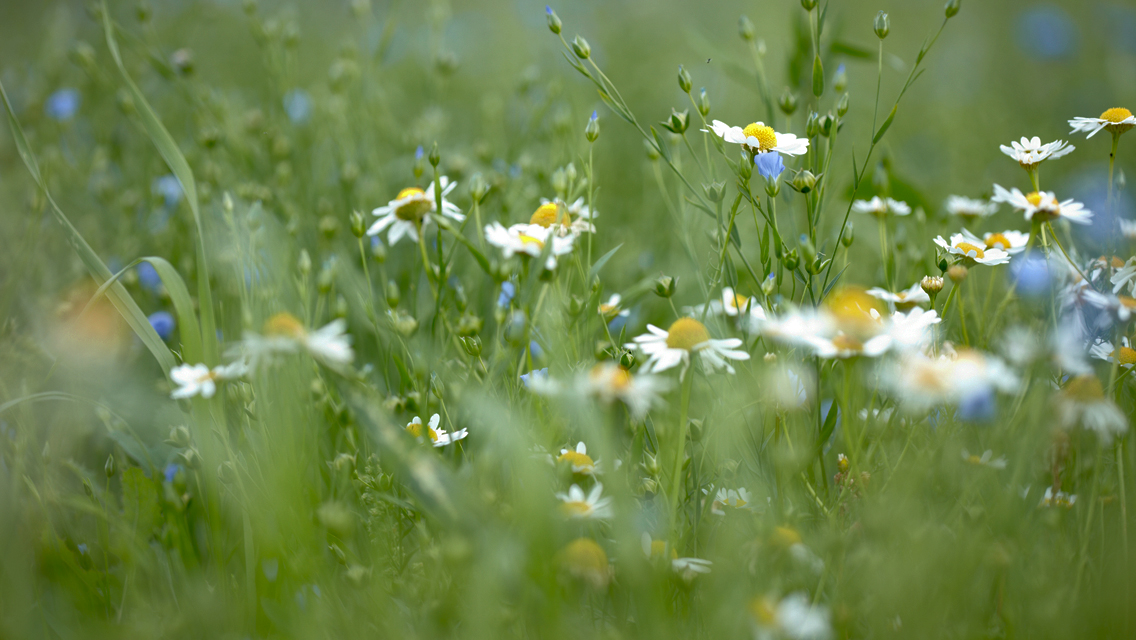
\includegraphics[width=12cm]{Daisy.jpg}| 的命令可以纳入图片.

如图 \ref{fig:1} 是一个纳入~jpg 图片的例子.

\begin{figure}[ht]
\centering
  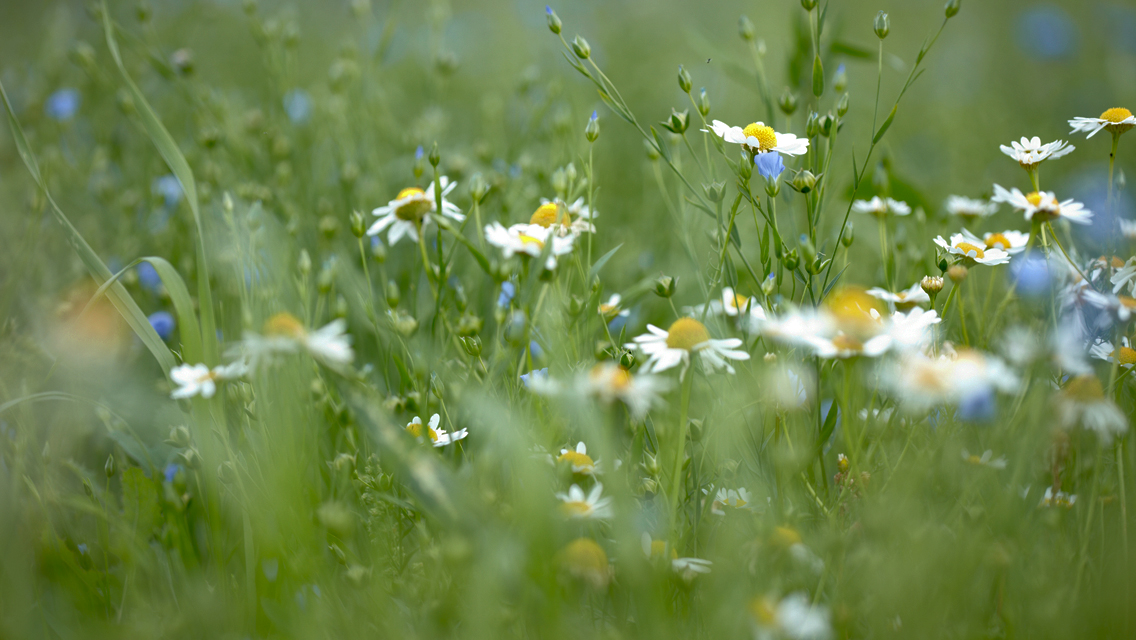
\includegraphics[width=\textwidth]{Daisy.jpg}
  \caption{一个彩色 jpg 图片的例子}
  \label{fig:1}
\end{figure}

表格问题, 建议使用``三线表'', 如表 \ref{tab:1}.

\begin{table}[ht]
\centering
\caption{一般三线表}
\label{tab:1}
    \begin{tabular}{c c c c c c c c c c c}
    \hline
    123 & 4  & 5  & 123 & 4 & 5123 & 4 & 5 & 123 & 4 & 5\\
    \hline
    67 & 890 & 13 & 123 & 4 & 5123 & 4 & 5 & 123 & 4 & 5\\
    67 & 890 & 13 & 123 & 4 & 5123 & 4 & 5 & 123 & 4 & 5\\
    67 & 890 & 13 & 123 & 4 & 5123 & 4 & 5 & 123 & 4 & 5\\
    \hline
    \end{tabular}
\end{table}

%\begin{table}[h]
%  \centering
%  \caption{调整线宽的三线表}\label{tab:2}
%    \begin{tabular}{c c c c c c c c c c c}
%    \hlinewd{0pt}
%    姓名: &&&&年龄: &&&& 性别:\\
%    \hlinewd{1.5pt}
%    123 & 4  & 5  & 123 & 4 & 5123 & 4 & 5 & 123 & 4 & 5\\
%    \hlinewd{1pt}
%    67 & 890 & 13 & 123 & 4 & 5123 & 4 & 5 & 123 & 4 & 5\\
%    67 & 890 & 13 & 123 & 4 & 5123 & 4 & 5 & 123 & 4 & 5\\
%    67 & 890 & 13 & 123 & 4 & 5123 & 4 & 5 & 123 & 4 & 5\\
%    \hlinewd{1.5pt}
%    \end{tabular}
%\end{table}








\chapter{其他事项}
以下是广告时间, 插播一段广告:
\begin{itemize}
    \item 插图的制作, 建议 pgf.
          pgf 的长处是源文件直接植入~\TeX~文档, 管理起来非常方便.
    这里有我写的一个关于初次使用~pgf~的帖子:\\    \url{http://bbs.ctex.org/forum.php?mod=viewthread&tid=30480}.
    \item 生成参考文献, 建议使用~BibTeX.  这里有我写的一个文档: \\
    \url{http://bbs.ctex.org/forum.php?mod=viewthread&tid=26056}.

      {\kaishu 使用 BibTeX{} 做参考文献时,
      借助 EndNote 或者 NoteExpress, 可以非常漂亮简单地解决 bib 文件的录入问题.
      NoteExpress 在校图书馆网站有正版软件提供下载.
      当然 EndNote 本身就是 Thomson Corporation 推出的(和 SCI 搜索引擎是同一家公司),
      和多个重要文献搜索引擎有良好的功能配合.

      Google 学术搜索也提供了文献的 bib 格式.
      录入参考文献时, 偶尔用一用 Google 学术搜索, 还可以核查或减少录入的错误, 并减少录入的工作量.}
     \item 幻灯片的制作, 建议使用~Beamer. 这里有我写的一个模板, 谨供参考:\\
    \url{http://bbs.ctex.org/forum.php?mod=viewthread&tid=27695}.
\end{itemize}

\chapter{杭州电子科技大学研究生学位论文格式统一要求}


% 不建议使用下列的参考文献使用方法,建议使用bib文件
%%%=== 参考文献 ========%%%
\cleardoublepage\phantomsection
\addcontentsline{toc}{chapter}{参考文献}
\begin{thebibliography}{000}\zihao{5}

  \bibitem{r1} 作者, 文章题目, 期刊名, 年份(期数): 起止页码

  \bibitem{r2} 作者, 书名, 年份, 版次, 出版地: 出版单位, 起止页码

  \bibitem{r3} 邓建松等, 《\LaTeXe~科技排版指南》, 科学出版社

  \bibitem{r4} 吴凌云, 《CTeX~FAQ (常见问题集)》, \textit{Version~0.4}, June 21, 2004

  \bibitem{r5} Herbert Vo\ss, Mathmode, \url{http://www.tex.ac.uk/ctan/info/math/voss/mathmode/Mathmode.pdf}.

\end{thebibliography}



\backmatter
% !Mode:: "TeX:UTF-8"

%%% 此部分内容:  (1) 致谢 

%%%%%%%%%%%%%%%%%%%%%%%
%%% --------------- 致谢 ------------- - %%%
%%%%%%%%%%%%%%%%%%%%%%%
\acknowledgement


感谢你, 感谢他和她, 感谢大家.


%%%%%%%%%%%%%%%%%%%%%%%%%%%%%%%%%%%%%%%
%%%%%%%--判断是否需要空白页-----------------------------
  \iflib
  \else
  \newpage
  \cleardoublepage
  \fi
%%%%%%%-------------------------------------------------

\chapter{附录}
论文:





 %%%致谢

\cleardoublepage
\end{document}



